\documentclass{beamer}

\usepackage{color}
\usepackage{graphicx}
\usepackage{amsmath}

\newcommand{\blue}[1]{\textcolor{blue}{#1}}
\newcommand{\red}[1]{\textcolor{red}{#1}}
\newcommand {\bmu} {\mbox{\boldmath$\mu$}}

\setbeamertemplate{frametitle}[default][center]

\begin{document}

\begin{frame}
\begin{center}
\blue{\Large\bf Investigation of Neoclassical Tearing Mode}\\[1ex]
 \blue{\Large\bf Detection by ECE Radiometry in ITER}\\[1ex]
 \blue{\Large\bf via Asymptotic Matching}\\[1ex]
 \blue{\Large\bf Techniques}\,\footnote{arXiv:2506.05553}\\[4ex]
Richard Fitzpatrick\\[2ex]
{\em Institute of Fusion Studies, Department of Physics},\\[0.5ex] {\em University of Texas at Austin}
\vspace{4cm}
\end{center}
\end{frame}

\begin{frame}
\frametitle{Neoclassical Tearing Modes}
 
\begin{itemize}
\item ITER needs to avoid disruptions.
\item \textcolor{red}{Neoclassical tearing modes} (NTMs) are main cause of disruptions in ITER-relevant discharges in present-day tokamaks.
\item NTMs can be stabilized by means of localized \textcolor{red}{electron cyclotron current drive} (ECCD) that is targeted at one of  O-points of  NTM
island chain. 
\item \textcolor{red}{Early detection} of NTM island chain, combined with \textcolor{red}{accurate location} of O-points,  is key to successful disruption avoidance. 
\end{itemize}
\end{frame}

\begin{frame}
\frametitle{Electron Cyclotron Emission}
 
\begin{itemize}
\item \textcolor{red}{Electron cyclotron emission} (ECE) simultaneously  detects  NTM island chain, and
accurately determines its location. 
\item In existing synthetic ECE diagnostics,  a single-harmonic, radially-symmetric, NTM island chain, centered on 
rational surface, is
crudely inserted into plasma equilibrium. 
\item In reality, an NTM consists of \textcolor{red}{multiple} helical harmonics. 
\item Harmonics with  same toroidal mode number as  NTM, but different poloidal mode numbers, are
coupled \textcolor{red}{linearly} via toroidicity and flux-surface shaping throughout  plasma. 
\item Harmonics whose poloidal and toroidal mode numbers are in  same ratio as those of  NTM are coupled \textcolor{red}{nonlinearly} in  immediate vicinity of island chain. 
\item NTM island chains are \textcolor{red}{radially asymmetric} due to mean gradient in tearing eigenfunction at rational surface. 
\end{itemize}
\end{frame}

\begin{frame}
\frametitle{Determining Magnetic Structure of NTM}
 
\begin{itemize}
\item  In \textcolor{red}{asymptotic matching} approach, plasma divided into \textcolor{red}{outer region}, that comprises most of plasma, and \textcolor{red}{inner region} that is localized in vicinity of NTM rational surface. 
\item Tearing perturbation in outer region determined by solving linearized, marginally-stable,  ideal-MHD  equations in full toroidal geometry (using TJ toroidal tearing mode code). 
\item Tearing perturbation in inner region consists of nonlinear, radially-asymmetric, island equilibrium.
\item Solutions in inner and outer regions asymptotically matched to one another at boundary between two regions to determine properties of island chain (e.g., radial asymmetry) in terms of
tearing eigenfunction in outer region. 
\end{itemize}

\end{frame}

\begin{frame}
\frametitle{Determining Electron Temperature Perturbation}
 
\begin{itemize}
\item No change in topology of magnetic flux-surfaces in outer region. Electron temperature assumed to be passively convected by plasma. Hence,
perturbed temperature is minus product of radial plasma displacement and equilibrium temperature gradient.
\item In inner region, electron temperature assumed to be constant on island magnetic flux-surfaces. Temperature profile determined by solution of \textcolor{blue}{$\langle \nabla^2 T_e\rangle=0$}, where
\textcolor{blue}{$\langle\cdots\rangle$} denotes island  flux-surface average.
\item Global temperature profile determined by asymptotically matching temperatures in inner and outer region at boundary between two regions. Determines reduction in core temperature due to island chain.
\end{itemize}

\end{frame}

\begin{frame}
\frametitle{Example Plasma Equilibrium}
 
\begin{center}
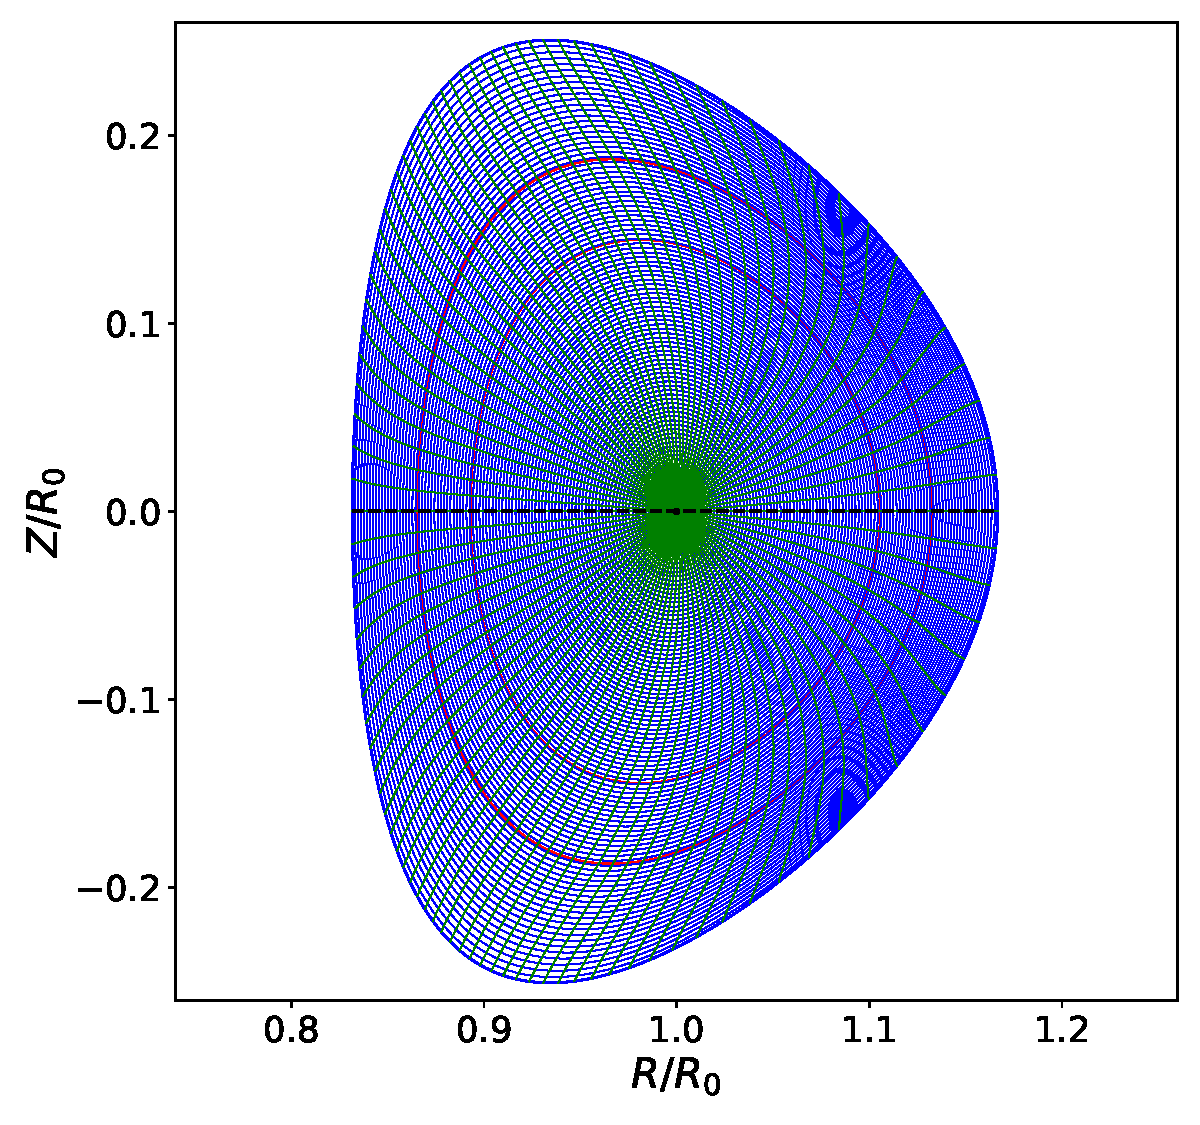
\includegraphics[width=0.55\textwidth]{../Fig1.pdf}
\end{center}
\begin{itemize}
\item Red curves show locations of \textcolor{blue}{$3,2$} and \textcolor{blue}{$2,1$} rational surfaces. 
\item Dashed line shows ECE measurement chord. 
\end{itemize}
\end{frame}

\begin{frame}
\frametitle{Asymmetric Magnetic Island}
 
\begin{center}
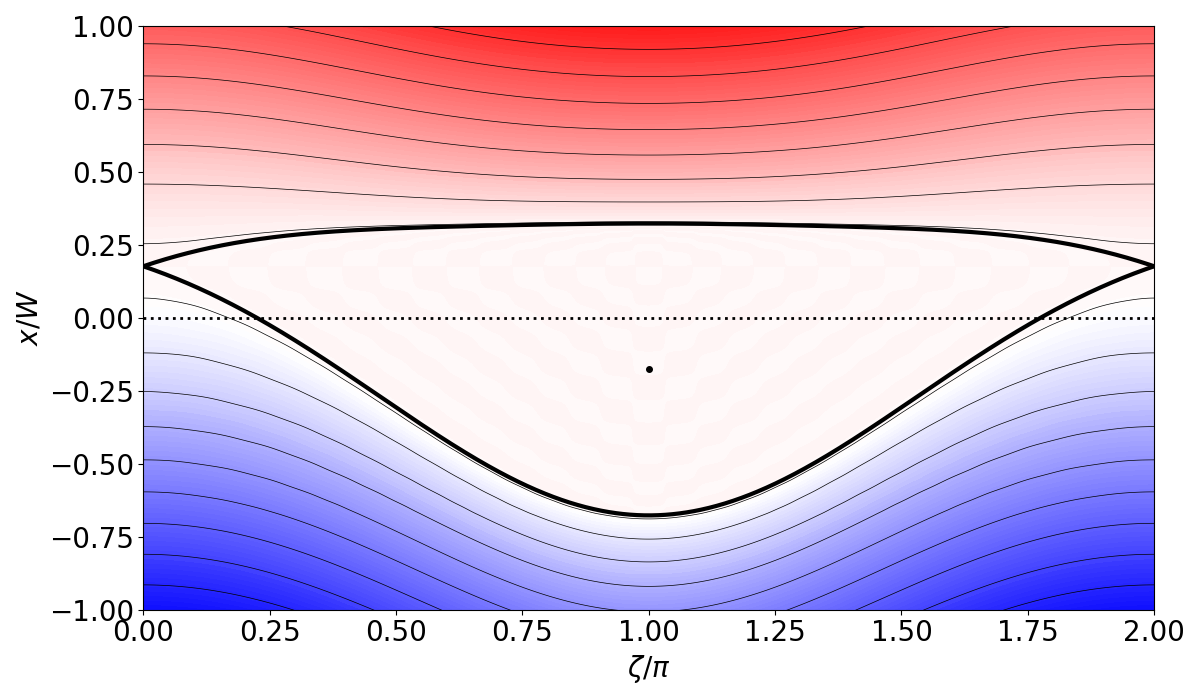
\includegraphics[width=0.7\textwidth]{../Fig7.png}
\end{center}
\begin{itemize}
\item \textcolor{blue}{$x=r-r_s$}, \textcolor{blue}{$\zeta = m\,\theta-n\,\phi$}, and \textcolor{blue}{$W$} is island width. Thick curve: island separatrix. Dot: island O-point. Dashed line: 
rational surface. Contours show electron temperature distribution.
\item Note that island O-point, which is true ECCD target, is shifted radially inward from rational surface. 
\end{itemize}
\end{frame}

\begin{frame}
\frametitle{Perturbed Electron Temperature}
 
\begin{center}
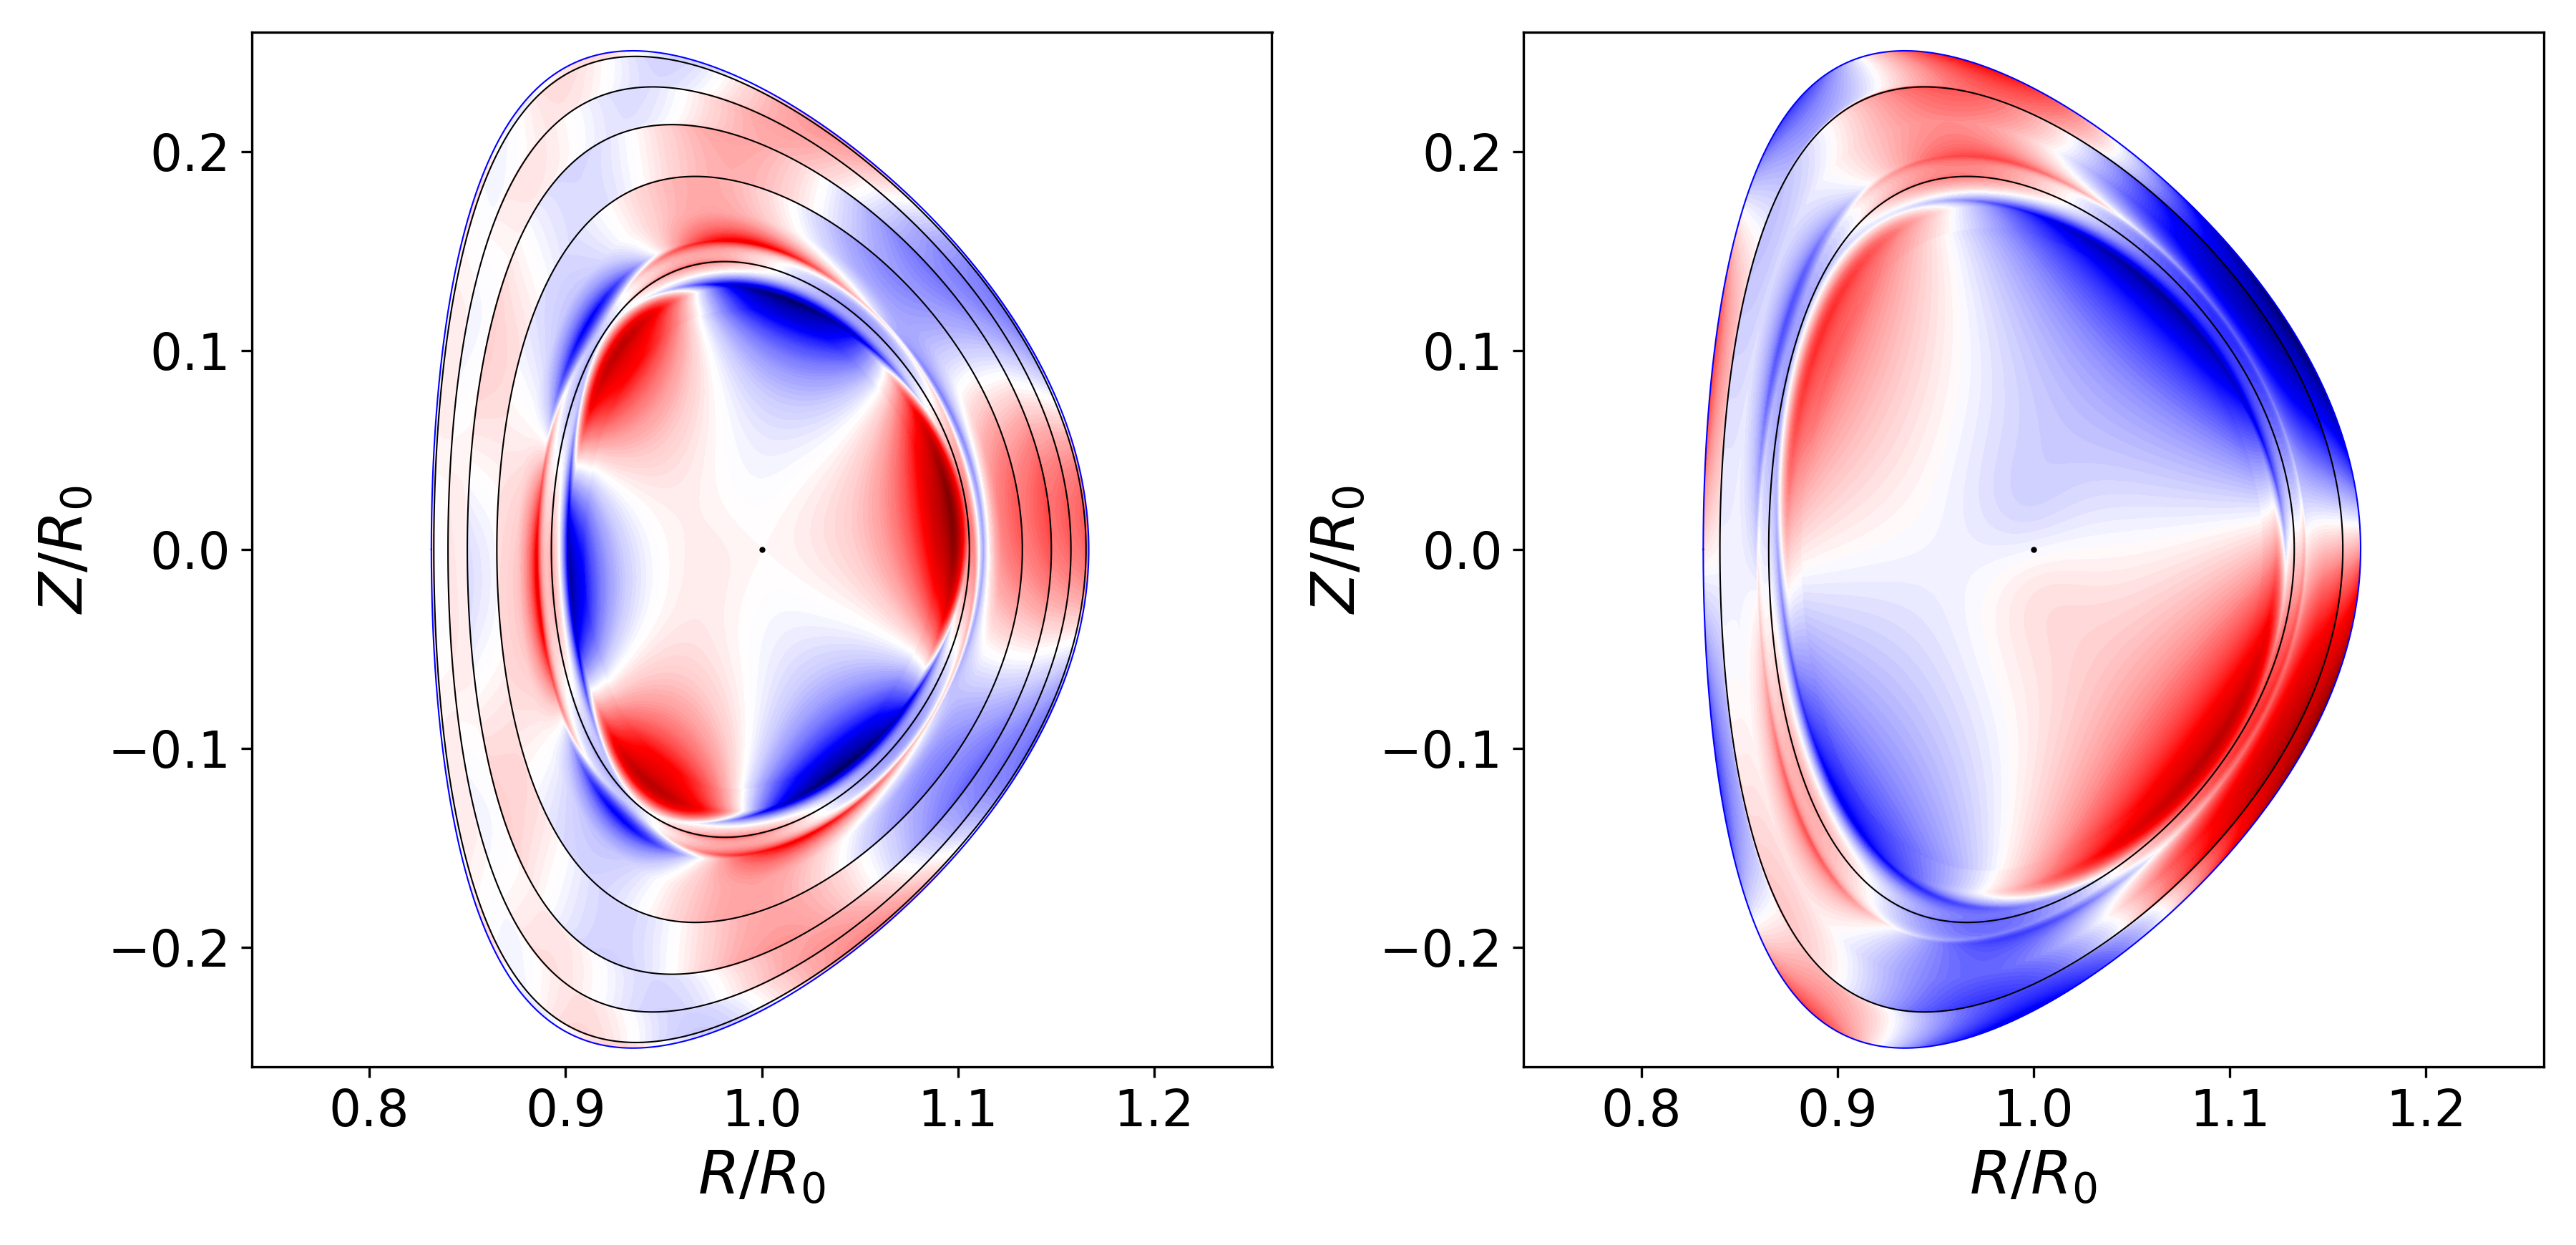
\includegraphics[width=0.85\textwidth]{../Fig13.png}
\end{center}
\begin{itemize}
\item Left/right panels: \textcolor{blue}{$3,2$}/\textcolor{blue}{$2,1$} NTMs. Black curves: toroidally coupled rational surfaces. Black dot: magnetic axis. 
\item Realistic temperature perturbation associated with NTM is surprisingly complicated.   
\end{itemize}
\end{frame}

\begin{frame}
\frametitle{Total Electron Temperature}
 
\begin{center}
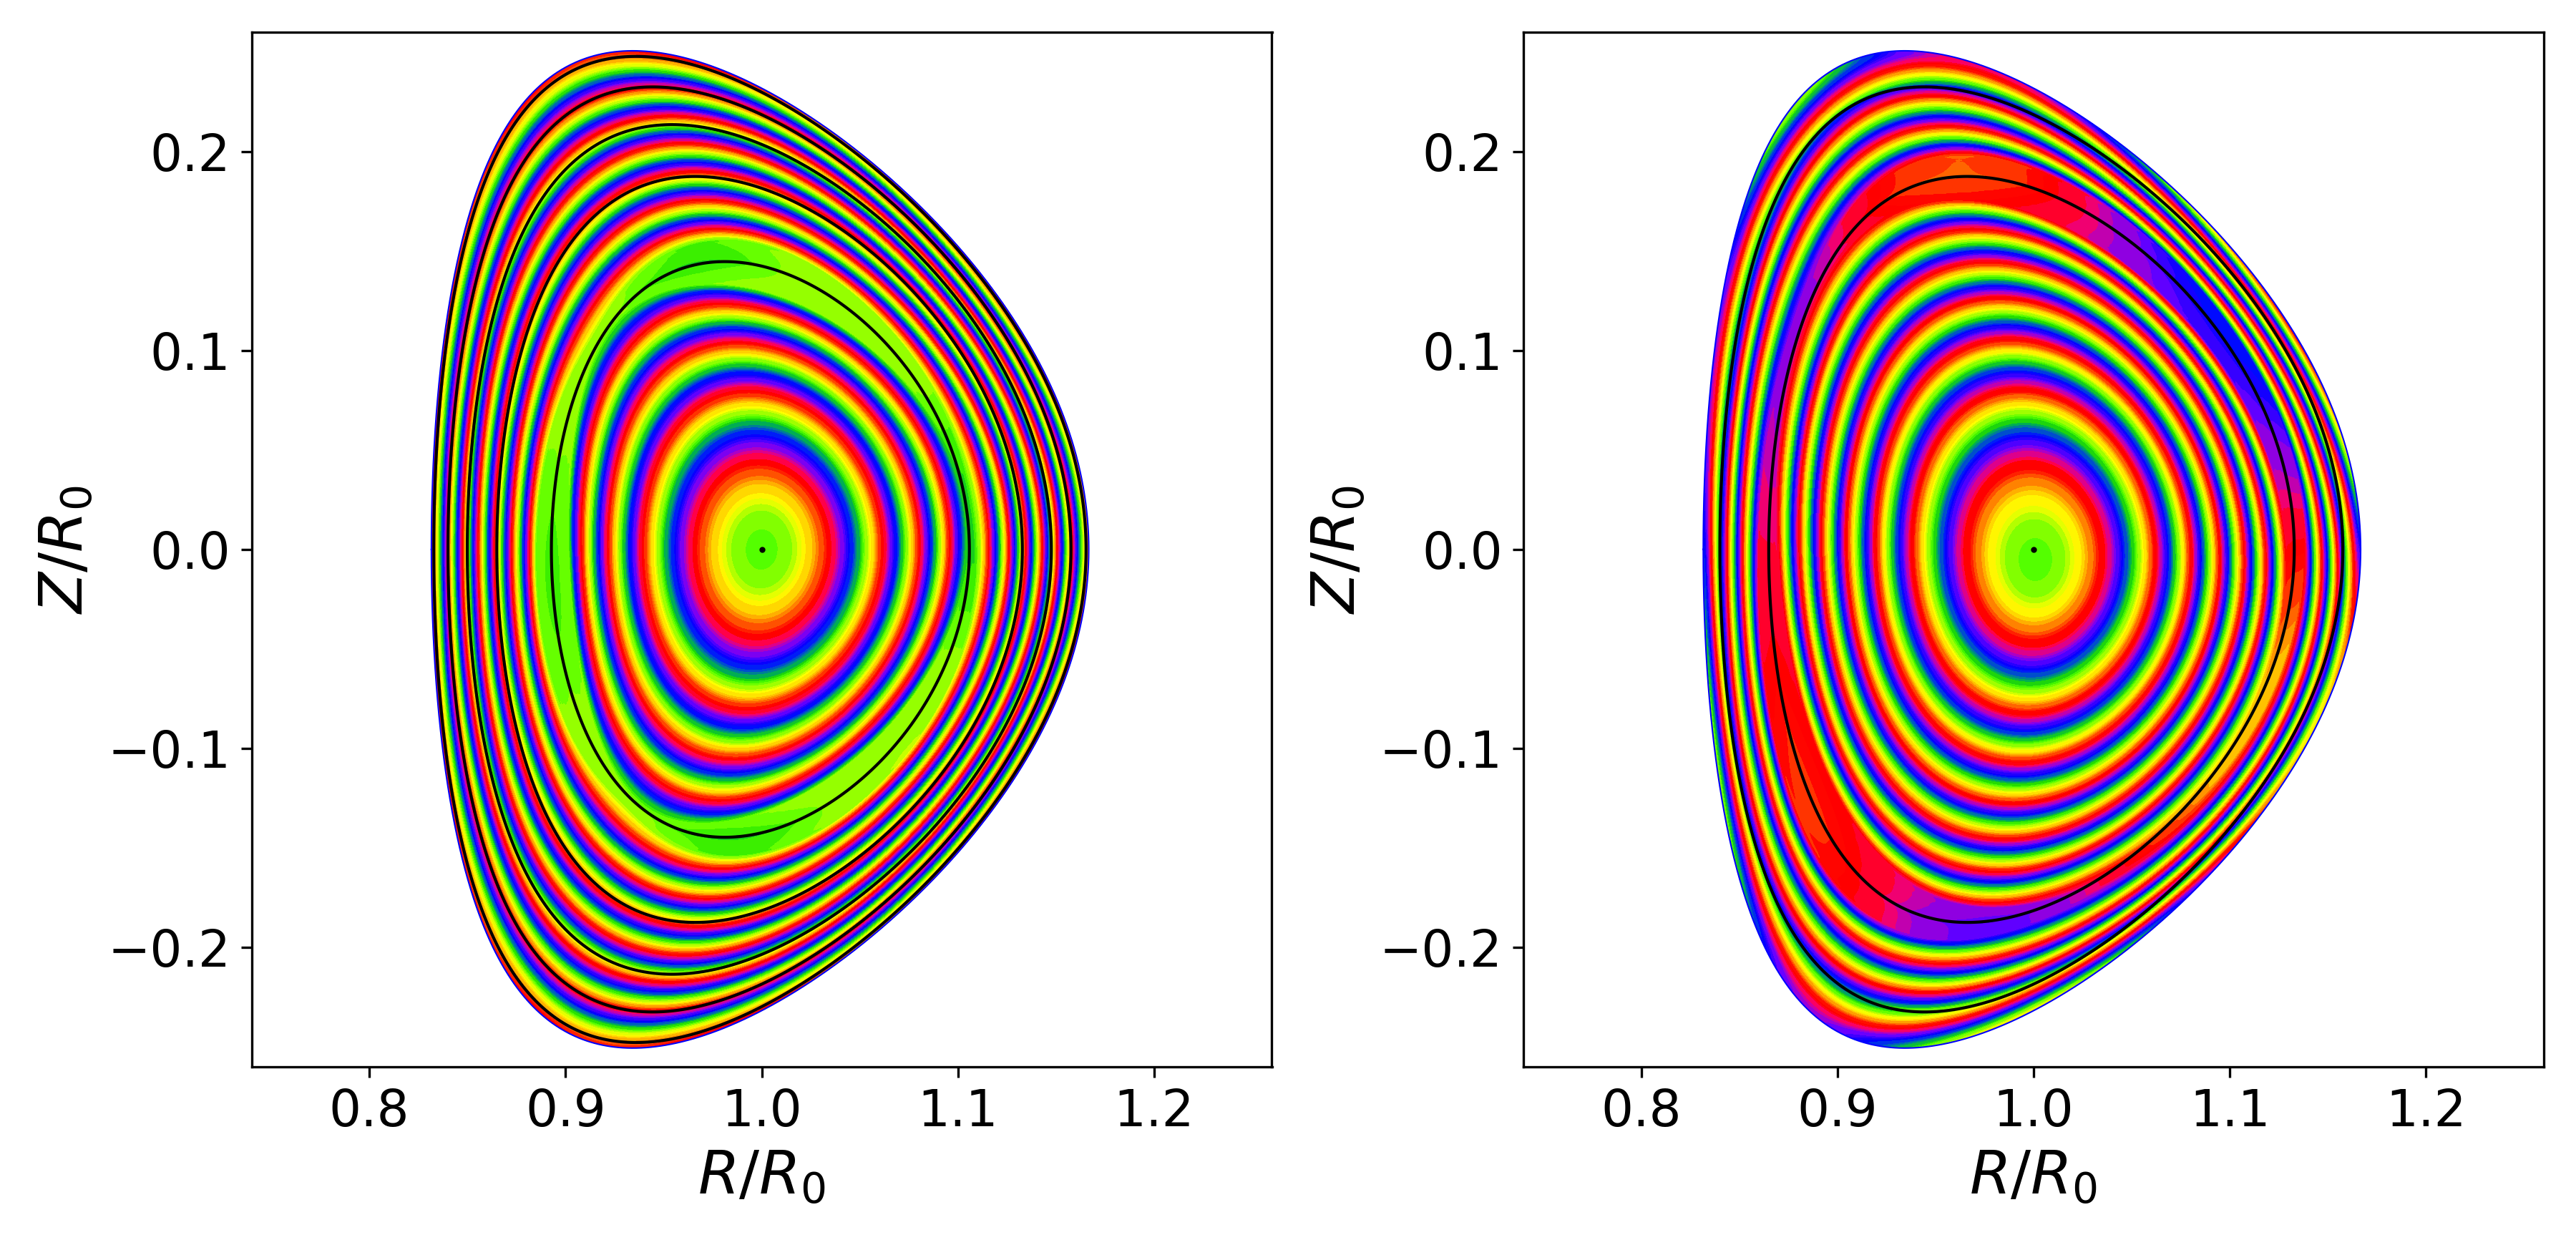
\includegraphics[width=0.85\textwidth]{../Fig14.png}
\end{center}
\begin{itemize}
\item Nevertheless, when perturbed electron temperature added to equilibrium temperature, result is appropriate helical flat-spot at NTM rational surface. 
\end{itemize}
\end{frame}

\begin{frame}
\frametitle{ECE Signal - I}
 
 \begin{itemize}
 \item In optically thick plasma, intensity of ECE emission directly proportional to electron temperature.
 \item Angular frequency of \textcolor{blue}{$j$}th harmonic ECE signal is
 $$
 \textcolor{blue}{\omega = \frac{j\,{\mit\Omega}_0\,R_0}{R}\left[1-\left(\frac{v}{c}\right)^2\right]^{1/2}},
 $$
 where $\textcolor{blue}{{\mit\Omega}_0=e\,B_0/m_e}$, $\textcolor{blue}{B_0}$ is on-axis toroidal magnetic field-strength,  \textcolor{blue}{$R_0$} is major radius of magnetic axis, and \textcolor{blue}{$v$}
 is electron speed. 
 \item Let 
 $$
 \textcolor{blue}{R_\omega(\omega) = \frac{j\,{\mit\Omega}_0\,R_0}{\omega}}
 $$
be the major radius from which ECE of frequency \textcolor{blue}{$\omega$} is emitted  in  absence of relativistic mass increase. \textcolor{blue}{$R$}
is actual major radius from which signal emitted. 
\end{itemize}
 \end{frame}
 
\begin{frame}
\frametitle{ECE Signal - II}
 
\begin{itemize}
 \item Distribution of electron speeds is
$$
\textcolor{blue}{f(v)= A\,v^2\,{\rm exp}\left(-\frac{1}{\theta_\omega}\left[1-\left(\frac{v}{c}\right)^2\right]^{-1/2}\right)},
$$
where
\textcolor{blue}{$\theta_\omega(\omega) = T_e(R_\omega)/(m_e\,c^{\,2})\ll 1$}. 

\item Can define 
$$
\textcolor{blue}{F(R,R_\omega) = \left[1-\left(\frac{R}{R_\omega}\right)^2\right]\exp\!\left(-\frac{1}{\theta_\omega}\,\frac{R_\omega}{R}\right)}.
$$

\item Electron temperature measured by  ECE diagnostic is  convolution of actual signal, \textcolor{blue}{$T_e(R)$},  and function \textcolor{blue}{$F(R,R_\omega)$}:
$$
\textcolor{blue}{T_e(R_\omega) = \frac{\int_{R_{\rm min}}^{R_\omega} T_e(R)\,F(R,R_\omega)\,dR}  {\int_{R_{\rm min}}^{R_\omega} F(R,R_\omega)\,dR}}.
$$
 \end{itemize}
 \end{frame}
 
 \begin{frame}
\frametitle{ECE Signal - III}
 
\begin{itemize}
\item Convolution specifies distortion of ECE signal due to relativistic mass increase. 
\item Taylor expanding: 
\begin{align*}
\textcolor{blue}{T_e(R_\omega)}&\textcolor{blue}{~= T_e(R_\omega) - 2\,\theta_\omega\left(1-\frac{13}{2}\,\theta_\omega\right) R_\omega\,\frac{d T_e(R_\omega)}{dR}}\\[0.5ex]
&\phantom{=}\textcolor{blue}{+ 3\,\theta_\omega^{\,2}\,R_\omega^{\,2}\,
\frac{d^2 T_e(R_\omega)}{dR^2} + {\cal O}(\theta_\omega^{\,3})}.
\end{align*}
\item To first order  in \textcolor{blue}{$\theta_\omega$}, 
measured temperature profile is \textcolor{blue}{$T_e[R_\omega\,(1-2\,\theta_\omega)]$}: i.e.,  measured profile shifted outward in major radius 
distance \textcolor{blue}{$2\,\theta_\omega\,R_\omega$}. 
\item To second order,  measured profile  smeared out in major radius. 
\end{itemize}
\end{frame}

\begin{frame}
\frametitle{Synthetic ECE Diagnostic}
 
 \begin{center}
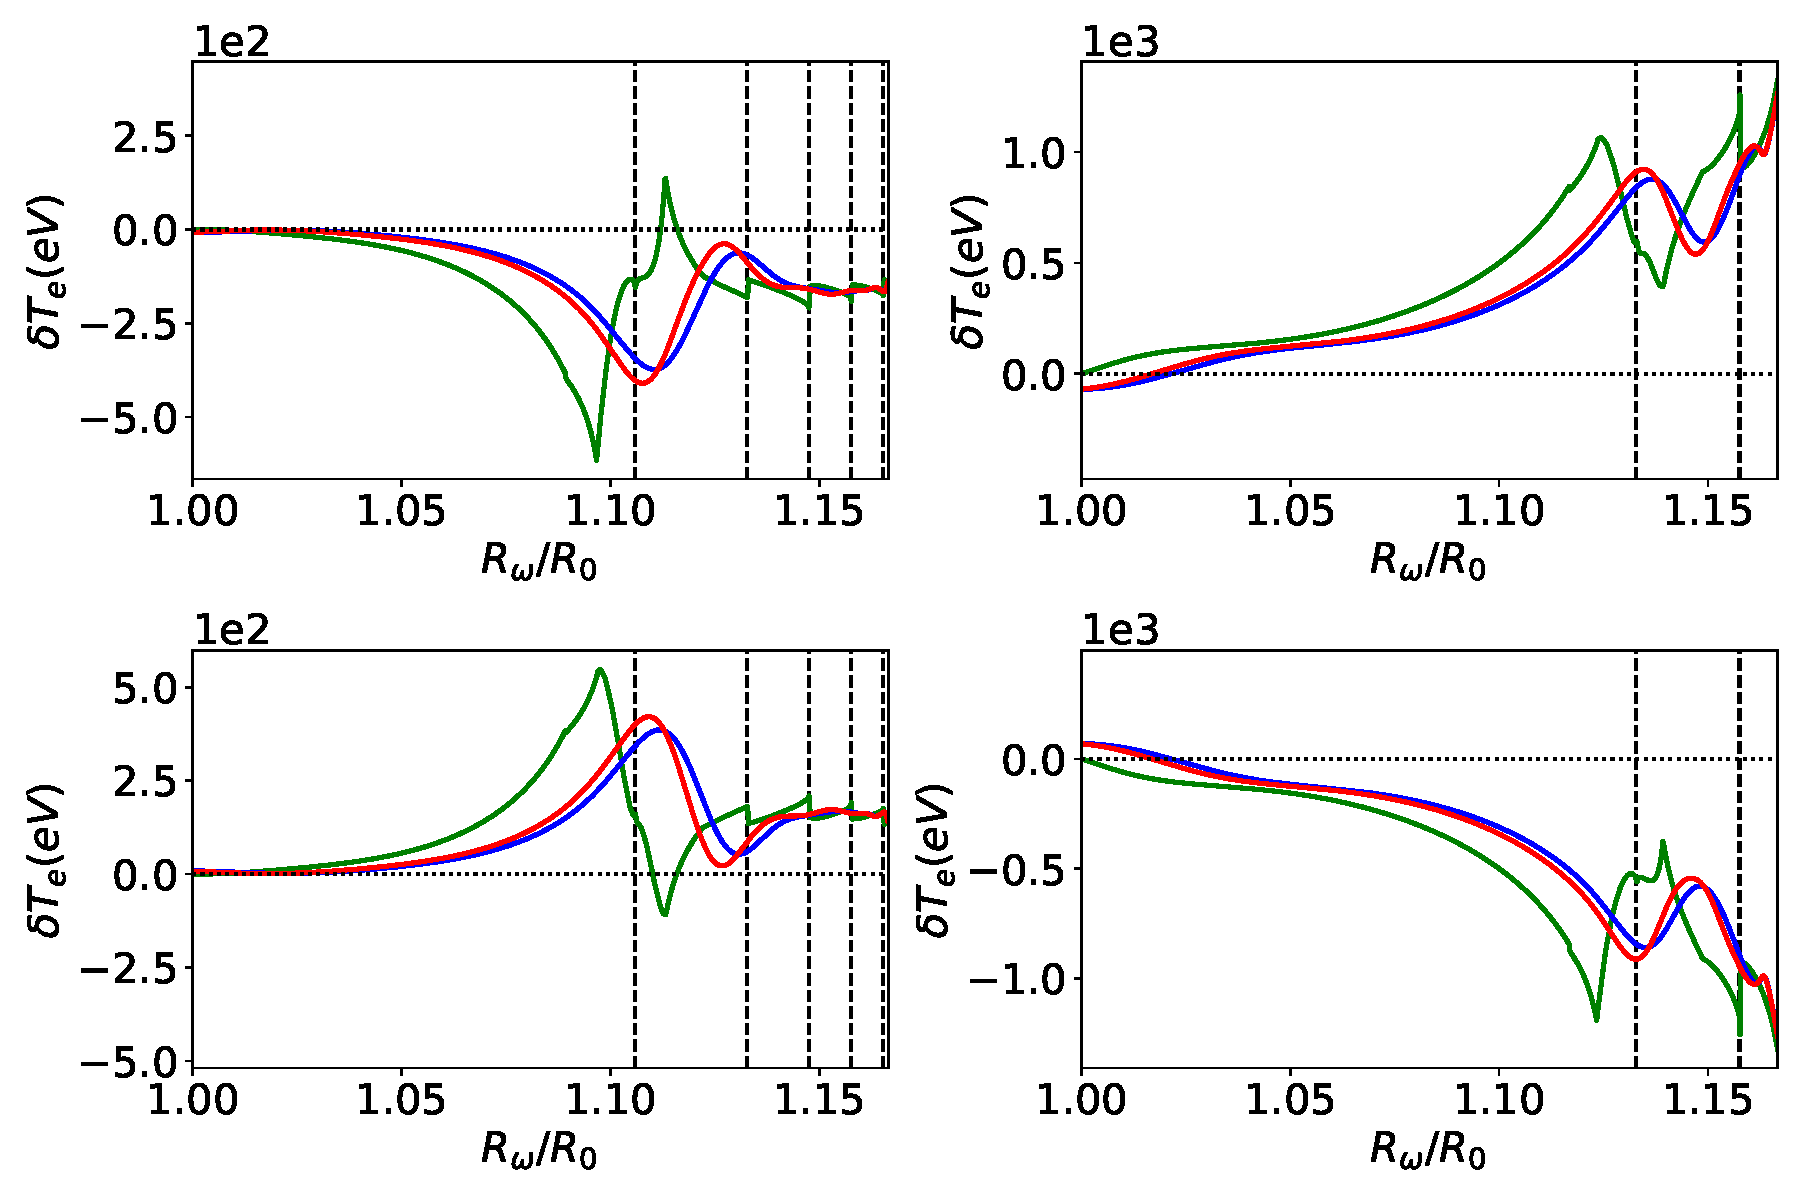
\includegraphics[width=0.65\textwidth]{../Fig16.pdf}
\end{center}

\begin{itemize}
\item Left/right-panels: \textcolor{blue}{3,2}/\textcolor{blue}{2,1} NTMs. Top/bottom panels: two different toroidal angles. Red/blue curves: distorted /undistorted ECE signals. Dashed lines: rational surfaces. 
\item Relativistic mass increase shifts inferred location of ECE signal outward in major radius, and also smears out signal. 
\end{itemize}
 \end{frame}
 
\begin{frame}
\frametitle{Synthetic Berrino Algorithm}
 
\begin{center}
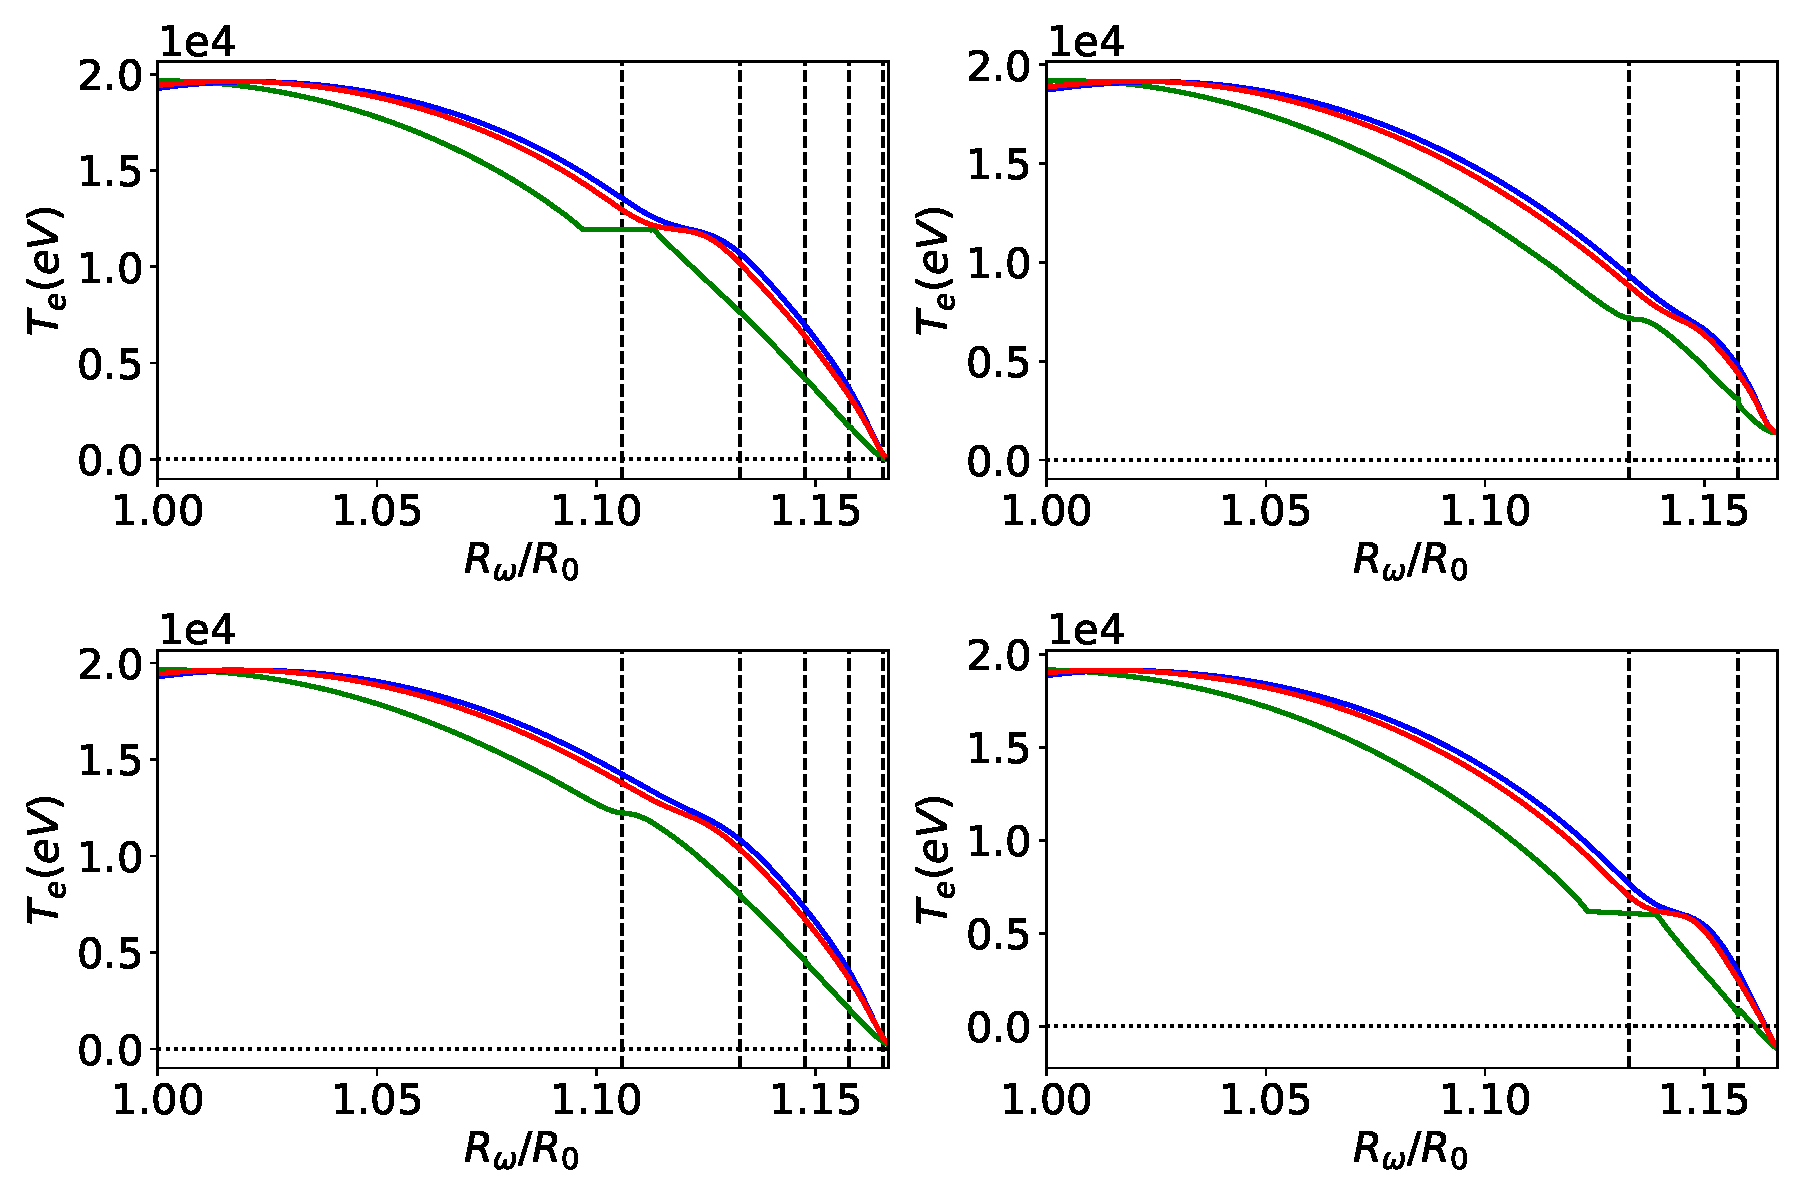
\includegraphics[width=0.65\textwidth]{../Fig17.pdf}
\end{center}

\begin{itemize}
\item Synthetic Berrino algorithm (radial gradient of ECE signal averaged over toroidal angle) gives clear signal for NTM islands whose widths are as small as \textcolor{blue}{1\%} of minor radius. 
\item Minimum of Berrino signal (which is usually taken as target radius for ECCD) shifted outward in major radius due to relativistic mass increase. 
\end{itemize}

\end{frame}

\begin{frame}
\frametitle{Conclusions}
 
\begin{itemize}
\item Asymptotic matching techniques permit rapid and realistic calculation of ECE signal generated by an NTM. 

\item Asymptotic matching techniques can calculate magnetic, temperature, and density perturbations associated with tearing mode in
both linear and nonlinear regimes. 

\item As such, asymptotic matching techniques could be used to simulate any diagnostic used to study tearing modes. 
\end{itemize}
\end{frame}



\end{document}